\documentclass{article}


% if you need to pass options to natbib, use, e.g.:
%     \PassOptionsToPackage{numbers, compress}{natbib}
% before loading neurips_2023


% ready for submission
\usepackage[final, nonatbib]{neurips_2023}


% to compile a preprint version, e.g., for submission to arXiv, add add the
% [preprint] option:
%     \usepackage[preprint]{neurips_2023}


% to compile a camera-ready version, add the [final] option, e.g.:
%     \usepackage[final]{neurips_2023}


% to avoid loading the natbib package, add option nonatbib:
%    \usepackage[nonatbib]{neurips_2023}


\usepackage[utf8]{inputenc} % allow utf-8 input
\usepackage[T1]{fontenc}    % use 8-bit T1 fonts
\usepackage{hyperref}       % hyperlinks
\usepackage{url}            % simple URL typesetting
\usepackage{booktabs}       % professional-quality tables
\usepackage{amsfonts}       % blackboard math symbols
\usepackage{nicefrac}       % compact symbols for 1/2, etc.
\usepackage{microtype}      % microtypography
\usepackage{xcolor}         % colors

\usepackage[spanish, es-tabla]{babel}

\usepackage[pdftex]{graphicx}
\usepackage{pgf}
\usepackage{subcaption}
\graphicspath{{./graphs/}}

%% biblatex
\usepackage[style = numeric, backend = biber, sorting = none, doi = false, isbn = false, url = true]{biblatex}
% \usepackage[defernumbers = true, style = numeric, backend = biber, sorting = none, doi = false, isbn = false, url = true]{biblatex}
% \usepackage[style = numeric, backend = biber, sorting = none]{biblatex}    % REFERENCIAS como section
\AtEveryBibitem{
    \clearfield{urlyear}
    \clearfield{urlmonth}
} % Do not show the "(visited on <date>)" on the references
\DefineBibliographyStrings{spanish}{}
\usepackage{csquotes}
\addbibresource{./dmcyt.bib}
\renewcommand*{\bibfont}{\fontsize{9}{12}\selectfont}



\title{Grafos en neurociencias (pre TP2)}

\author{
  Víctor A.~Bettachini\\ %\thanks{Use footnote for providing further information about author (webpage, alternative address)---\emph{not} for acknowledging funding agencies.} \\
  Datamining en ciencia y tecnología 2023\\
  Especialización en Explotación de Datos y Descubrimiento del Conocimiento\\
  \texttt{bettachini@gmail.com}
}


\begin{document}


\maketitle


\begin{abstract}
?
\end{abstract}


% Enunciado
% Se sugiere realizar la entrega en formato latex, pero en este caso va a ser optativo (en el TP ya es obligatorio, sugerimos que lo usen de práctica). Pueden acceder a formatos de distintas conferencias a través de Overleaf, en particular les sugerimos el formato de NeurIPS que es una de las conferencias más importantes en IA.
% Se sugiere un máx de 4 carillas (mín 2), no se debe incluir código a menos que sea algo esencial que hayan desarrollado ustedes (es preferible en este caso incluir el pseudo-código). Aclaración: No vamos a corregir código en la entrega.
% El pre TP es individual.


% \section{Introducción}

\section{Materiales y métodos}

\paragraph{Datos}
Se registró la señal de resonancia magnética funcional (fMRI) bajo distintos estadíos del sueño en distintas parcializaciones del cerebro. 
Para segmentos temporales se calculó el coeficiente de correlación lineal entre sus medias \cite{tagliazucchi_large-scale_2013}.
Estos son los datos de entrada con que se genera una matríz de correlación a partir de la cual se generan los grafos que se analizan en este trabajo.

\paragraph{Recurso informático} 
Un cuaderno (notebook) Jupyter provisto por los docentes en el sitio web denominado ``Campus'' \cite{kamienkowski_curso_2023} es la plantilla donde se escribió código en lenguaje Python.
Este explotó funciones de las biblioteca NetworkX \cite{hagberg_exploring_2008}.



\subsection{Preprocesamiento de los datos}
% Cada actividad realizada se describe bajo los titulos que figuran en el enunciado del trabajo práctico publicado en el

\paragraph{Carga del conjunto de datos} 
Los archivos provistos corresponden a los estadíos de sueño N1, N2, N3 y despierto (W) para 18 sujetos.
Estos estuvieron acompañados de una tabla que describe la denominacion y  ubicación espacial las regiones en que se parcializó el cerebro.



\section{Resultados}

\subsection{Manipulación de datos}

\paragraph{Matriz de correlación}
La matriz de adyacencia pesada que muestra la figura \ref{fg:matriz_correlación_pesada} corresponde a la condición de despierto para el sujeto número 2.

Para convertirle en una de adyacencia binaria con una densidad de enlaces \(\delta = 0.8\) se discriminaron sus pesos con un umbral \(0.77997\) obteníendose la matriz que muestra la figura \ref{fg:matriz_correlación_binaria}.

\begin{figure}[ht]
	\centering
	\begin{subfigure}[b]{0.4\textwidth}
		\includegraphics[width= \linewidth]{matriz_correlación}
		\caption{Pesada}
		\label{fg:matriz_correlación_pesada}
	\end{subfigure}
	\begin{subfigure}[b]{0.425\textwidth}
		\includegraphics[width= \linewidth]{matriz_correlación_binaria}
		\caption{Binaria}
		\label{fg:matriz_correlación_binaria}
	\end{subfigure}
	\caption{Matrices de correlación de las medias de las señales de las regiones parcializadas.
	}
	\label{fg:matriz_correlación}
\end{figure}


\paragraph{Grafo de la matriz de adyacencia binaria}
No es totalmente conectado. Hay tres componentes conectadas de 92, 5 y 2 nodos en tanto que los 17 restantes están aislados.
La distancia mínima entre nodos contabiliza cuantos intermedios deben atravesarse para ir de un nodo a otro.
Esta medida para los aislados no tiene sentido, por lo en este grafo no puede obtenerse una distancia media $d$ a lo fines de tener una media de que tan ``conectado'' se presenta el grafo.
Una medida númerica alternativa darla la densidad que cuantifica cuantos de los posibles enlaces están efectivmente presentes en el grafo.
Para el conjunto, no conectado, este valor parece bajo, $\approx 8\%$.
Y en el componente mayoritario, el de 92 nodos, este valor apenas se incrementa hasta un $\approx 12\%$. 


\paragraph{Eficiencia de conectividad}
La distancia mínima entre nodos contabiliza cuantos intermedios deben atravesarse para ir de un nodo a otro.
Un promedio de la inversa de esta distancia es una medida de la eficiencia de conectividad global del grafo, que para este caso resultó ser $\approx 0.389$.


\paragraph{Distribución de grado}
El número de enlaces por nodo, o grado $k$, se distribuye en forma dispar.
De un total de $534$ enlaces el grado mayor resultó $k_{máx} = 30$, y un relativamente alto promedio $\langle k \rangle \approx 9.207$ aunque no hay que olvidar que no participan aquí los nodos aislados.
El histograma de $k$ que muestra la figura \ref{fg:hist_k} que este $\langle k \rangle$ es representativo de la distribución.

En una medida similar a la densidad que cuenta la proporción de enlaces sobre los posibles puede hacerse algo similar calculando la proporción de cuantos de los posibles enlaces entre primeros vecinos efectivamente se realizan.
Esto se denomina coeficiente de agrupamiento (clustering) por nodo $C_i$, cuyo promedio para este grafo es $\langle C_i \rangle \approx 0.527$. 
Coloreando cada nodo según su $C_i$ y ubicandole por las coordenadas (y,z) en el cerebro se obtiene la figura \ref{fg:clustering}. 

\begin{figure}[ht]
	\centering
	\begin{subfigure}[b]{0.25\textwidth}
		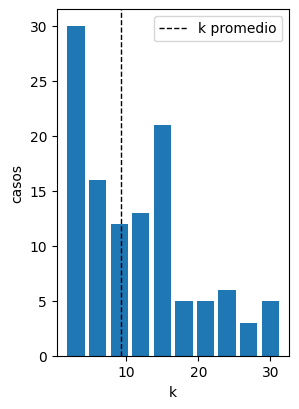
\includegraphics[width= \linewidth]{histograma_k}
		\caption{Histograma para $k$.
		}
		\label{fg:hist_k}
	\end{subfigure}
	\begin{subfigure}[b]{0.7\textwidth}
		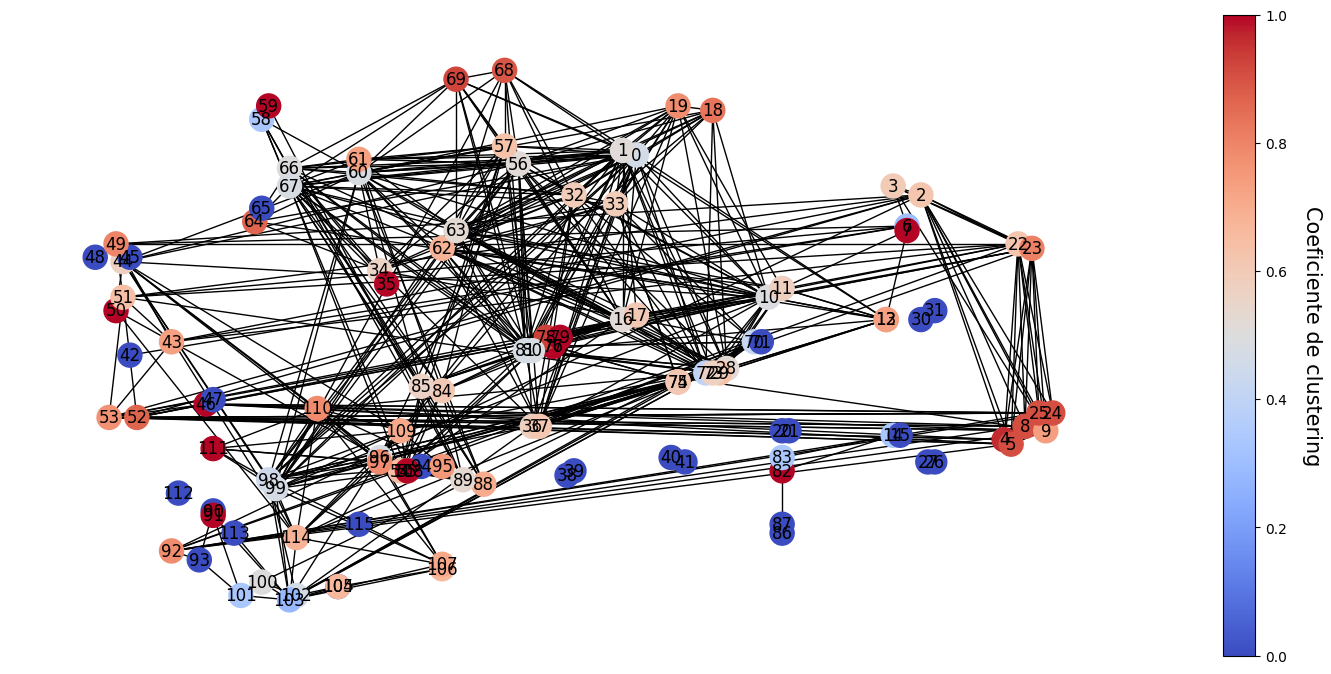
\includegraphics[width= \linewidth]{clustering}
		\caption{número de nodo $i$ y su $C_i$.
		}
		\label{fg:clustering}
	\end{subfigure}
	\caption{Distribución de grado y coeficiente de agrupamiento.
	}
	\label{fg:distribución_de_grado}
\end{figure}


\begin{figure}[ht]
  \centering
  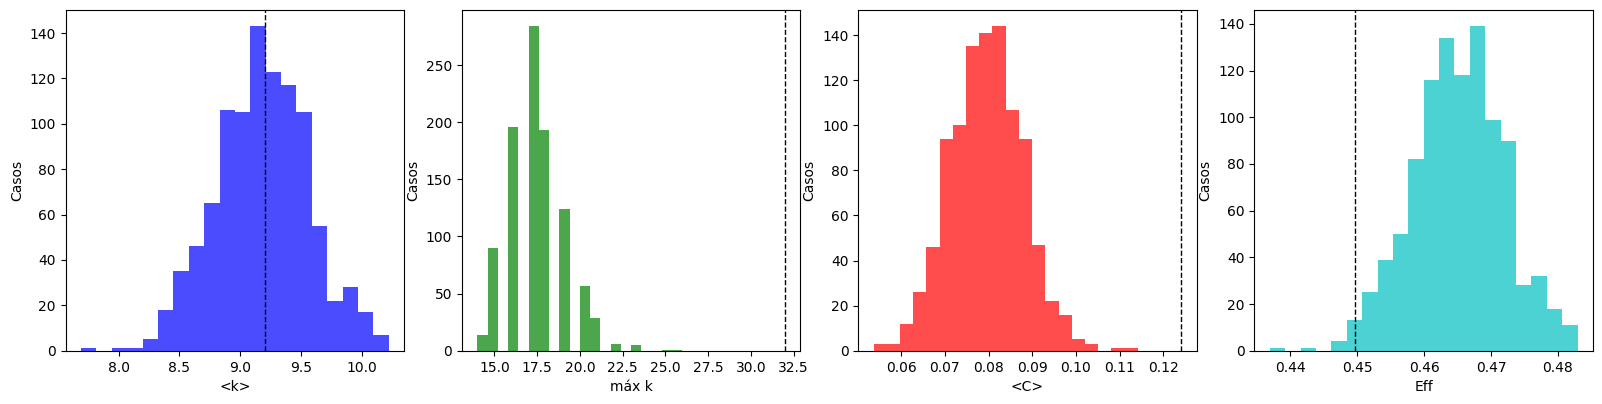
\includegraphics[width= \linewidth]{hist_poisson}
  \caption{Poisson
	}
	\label{fg:hist_poisson}
\end{figure}


\paragraph{Comparación con grafos propotípicos}



% \section{Discusión}

\printbibliography[title= Referencias, heading=bibintoc]

\end{document}
